\chapter{System do klasyfikacji elementów morometrycznych krwi}
\label{cha:system_do_klasyfikacji_elementow_morfologicznych}

\section{Przygotowanie bazy danych}
\label{przygotowanie_danych}

Baza danych zawiera 12500 zdjęć krwinek białych w formacie JPEG wykonanych pod mikroskopem. Pogrupowane są w cztery foldery według przynależności do klas, każdy po około 3000 ramek. Uwzględnione typy krwnek to neutrofil, eozynofil, limfocyt, monocyt. Zbiór został stworzony z 410 obrazów przez operację powiększania zbioru (ang. \textit{data augmentation}) \cite{database_kaggle}.

{\parindent0pt % disables indentation for all the text between { and }
Ramki wczytane bezpośrednio z bazy źródłowej do programu są w formacie RGB. Piksele oryginalnych obrazów mogą przyjmować wartości z zakresu od 0-255. Dla lepszego działania sieci neuronowej zaleca się normalizację wartości pikseli do małego zakresu, najlepiej 0-1 oraz ustandaryzowanie tak, aby można było traktować dane wejściowe jako rozkład Gaussa o średniej 0 i odchyleniu standadowym 1 (\ref{equ:standarisation}), \cite{standarisation}.

\begin{equation}
z =  \frac{x - \mu}{\sigma} 
\label{equ:standarisation}
\end{equation}
gdzie,
\begin{eqwhere}[2cm]
	\item[$x$] oryginalna wartość piksela,
	\item[$\mu$] średnia z wartości pikseli w ramce,
	\item[$\sigma$] odchylenie standardowe wartości pikseli w ramce,
	\item[$z$] wartość piksela po ustandaryzowaniu.
\end{eqwhere}
}

\subsection{Zastosowanie metody augmentacji danych}
W przypadku małych zbiorów danych, rozumianych jako zbiór liczący kilka tysięcy elementów często stosowaną praktyką jest poszerzanie zboru danych. Ma ona na celu bezpośrednio powiększenie ilości danych wprowadzanych do modelu, a pośrednio polepszenie rezultatów klasyfikacji. Jednym z korzystnych efektów tego działania jest redukcja zjawiska nadmiernego dopasowania (\textit{ang. overfiting}). Objawia się ona zmniejszeniem różnicy między błędem zbioru, na którym się trenuje model a błędem zbioru, na którym model jest testowany. Szczególnie dużą poprawę w tym aspekcie obserwuje się właśnie dla sieci typu CNN \cite{Wong2016UnderstandingDA}.

{\parindent0pt % disables indentation for all the text between { and }
Jednym ze sposobów transformacji jest elastczna deformacja w przestrzenii danych (\textit{ang. data-space elastic deformation}). Obrazy w oryginalnym zbiorze danych zostają poddane losowym transformacjom, z założeniem, że zachowane zostają informacje o przynależności do danej klasy. Daje najlepsze rezultaty w porównaniu do poszerzania w przestrzenii cech (\textit{ang. feature-space augmentation}) \cite{Wong2016UnderstandingDA}. Definiuje ona znormalizowany obszar losowego przemieszczenia \(u(x,y)\), który dla każdego piksela w obrazie \((x,y)\) definiuje wektor przemieszczenia \(R_w\) (\ref{equ:augmentation}), \cite{Wong2016UnderstandingDA}:

\begin{equation}
R_w = R_0 + \alpha u
\label{equ:augmentation}
\end{equation}
gdzie,
\begin{eqwhere}[2cm]
	\item[$R_w$] lokalizacja piksela w obrazie wyjściowym,
	\item[$R_0$] lokalizacja piksela w oryginalnym obrazie,
	\item[$\alpha$] wielkość przesunięcia w pikselach.
\end{eqwhere}
%Odległość półpauzy od lewego marginesu należy dobrać pod kątem najdłuższego symbolu (bądź listy symboli) poprzez odpowiednie ustawienie parametru tego środowiska (domyślnie: 2 cm).

Nie jest wskazane używanie zbioru powiększonego z użyciem dużych transformacji. Dla bazy MNIST przesunięcia \( \alpha \geq 8 \)  pikseli skutkuje w pewnej części przypadków utratą informacje o przynależności do danej klasy. Jest to definiowane jako brak zdolności do rozpoznania i zaklasfikowania danej ramki przez człowieka \cite{Wong2016UnderstandingDA}.

W przypadku rozpoznawania typów komórek augmentacja z zastosowaną zmianą skali może skutkować pogorszeniem dokładności klasyfikacji, gdyż na każdy rodzaj komórki ma swoją typową wielkość. Skorzystanie z tej cechy do nauczenia się rozpoznawania elementów z pewnością podnosi poziom precyzji działania algorytmu. Zaburzenie tej cechy przez manipulację skalą zdjęcia będzie skutkować utraceniem tej informacji. Zbiór danych zostanie powiększony, jednak stanie się to kosztem utraty pewnych pomocnych danych.

Baza danych użyta w pracy oryginalnie zawiera obrazy, będące wynikiem operacji powiększania zbioru. Oryginalna baza danych zawierała 410 obrazów krwinek białych. W wyniku powięszania zbiou powstała baza wkorzystywana w niniejszym projekcie. Z tego powodu nie jest wskazane dodatkowe przepowadzanie powiększania. Sumarcznie, użyta baza zawiera 12444 obrazy krwinek białych z czterech rozpatrywanych kategorii.
}

\subsection{Podział na podzbiory}

W celu wykorzystania danych do stworzenia sieci należy je podzielić na podzbiory: uczący - służący do wytrenowania sieci, walidacyjny - służący do nastrojenia sieci oraz testowy - użyty tylko raz na samym końcu gdy klasyfikator jest gotowy w celu sprawdzenia skuteczności sieci na nowych danych.

{\parindent0pt
Sposób podziału bazy danych na zbiory ma znaczący wpływ na jakość klasyfikatora, jaki można uzyskać. W przpadku przeznaczenia dużej ilości danych do treningu łatwiejsze będzie uzyskanie dobrej skuteczności na danych teningowych. Jednak nie da to pewności czy sieć zadziała poprawnie dla nowych danych, gdyż zbiory walidacyjny i testowy będą ograniczone. W sytuacji odwrotnej, przy użyciu dużej ilości danych do strojenia i testów sieć może nie nauczyć się odpowiedniej ilości różnorodnych wzorców, gdyż zbiór treningowy został ograniczony.

Początkowym podział bazy na zbiory został zrobion zgodnie z podejściem zastosowanym w rozdziale \ref{sec:section_kaggle_1}. Dzięki temu uzyskane wyniki będą mogły być porównywane.
}

\section{Zaproponowana struktura sieci neuronowej}
%narzędzie do rysowania sieci: http://alexlenail.me/NN-SVG/LeNet.html
%ResNet - spróbować wpiąć do mojej sprzężenie tak jak tutaj: https://medium.com/analytics-vidhya/cnns-architectures-lenet-alexnet-vgg-googlenet-resnet-and-more-666091488df5
Struktura sieci neuronowej bazuje na wybranych cechach zaczerpiętych z architektur VGGNet, U-Net oraz ResNet. VGGNet jest to architektura sieci kowolucyjnej opublikowanej przez Visual Geometry Group na Universitecie Oksfordzkim w 2014 roku \cite{VGG16_info}. Wytrenowana na 1.3 milionach obrazów treningowych dzielących się na 1000 klas uzyskała 92,7\% skuteczności na zbiorze testowym \cite{deep_learning_w_keras} \cite{VGG16_article_online}. Charakteryzuje się jednolitą budową i składa się jedynie z warstw konwolucyjnych przekładanych co dwie lub trzy warstwy redukcją maksymalizującą oraz trzech warstw gęsto połączonych, umieszczonych na końcu modelu (Rys. \ref{fig:vgg_16_stucture}). Najczęściej w literaturze występuje w wersjach z 16 (VGG16) i 19 (VGG19) warstwami konwolucyjnymi. 

\begin{figure}[h]
	\centering
	\centering
		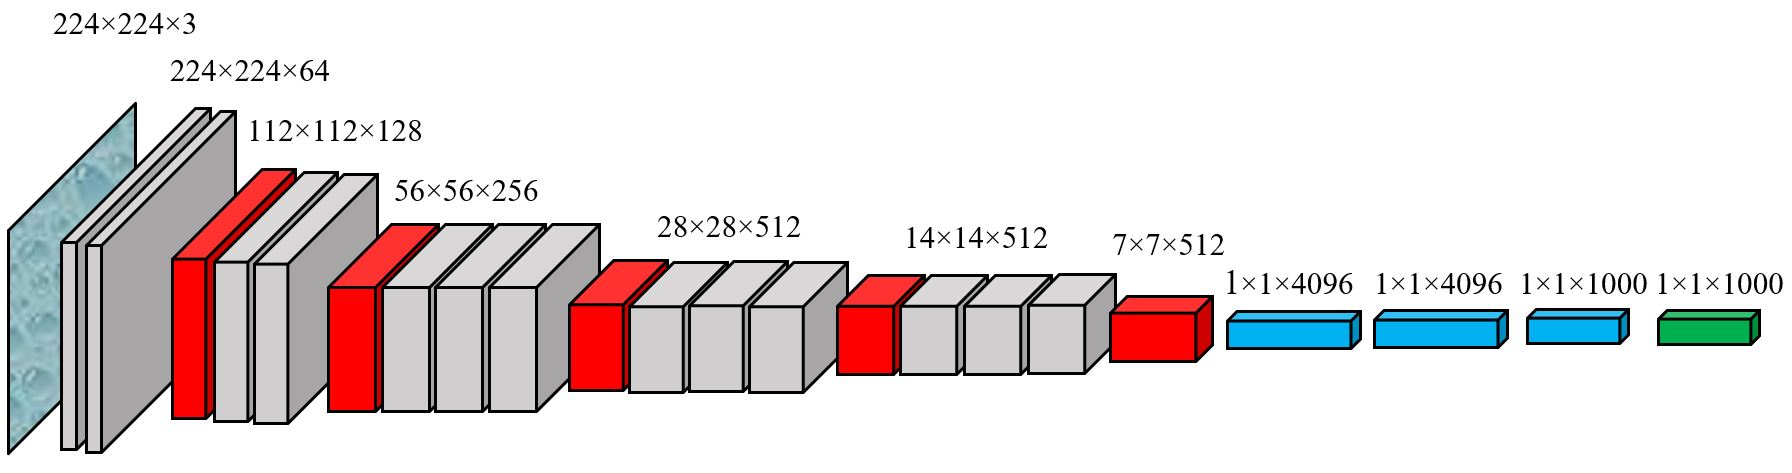
\includegraphics[scale=0.35]{VGG_16_structure}	
	\caption{Wizualizacja architektury sieci VGG16 \cite{VGG_16_structure}.}
	\label{fig:vgg_16_stucture}
	\label{fig:ann_visualisation}
\end{figure}

{\parindent0pt
Biblioteka Keras udostępnia przetrenowany model sieci VGG16. Z uwagi na bardzo dobre rezultaty uzyskane przy użyciu przenoszenia uczenia w rozdziale \ref{sec:section_kaggle_3} zdecydowano się na sprawdzenie jakie wyniki uzyska mniej skompikowany w budowie model. W tym celu rozmrożono trzy ostatnie warstwy konwolucyjne i ponownie wyuczono sieć na zdjęciach krwinek. Uzyskano dość dobre rezultaty na wszystkich zbiorach (\ref{tab:VGG16_acc}), a skuteczność klasyfikacji każdej klasy jest na podobnym poziomie (\ref{tab:VGG16_params_val}).

%VGG16_trainable_14:
 \begin{table}[h!]
\centering
\caption[Short Heading]{Skuteczność modelu w powtórzonym eksperymencie.}
\label{tab:VGG16_acc}
\begin{tabular}{|c|c|c|c|}
\hline
\textbf{typ zbioru}           & \textbf{treningowy} & \textbf{walidacyjny} & \textbf{testowy} \\ \hline
\textbf{skuteczność {[}\%{]}} & 99                  & 99                   & 71               \\ \hline
\end{tabular}
\end{table}

\begin{table}[h!]
\centering
\caption[Short Heading]{Parametry mierzące jakość klasyfikacji na zbiorze testowym.}
\label{tab:VGG16_params_val}
\begin{tabular}{|c|c|c|c|c|}
\hline
\textbf{Parametr}                               & \textbf{Precyzja} & \textbf{Czułość} & \textbf{Miara F1} & \textbf{Ilość próbek} \\ \hline
\textbf{klasa eozynofil (E)} & 0.24   & 0.32   & 0.27 & 623  \\ \hline
\textbf{klasa limfocyt (L)} & 0.22  & 0.22 & 0.22  & 620  \\ \hline
\textbf{klasa monocyt (M)} & 0.20   & 0.07    & 0.10  & 620  \\ \hline
\textbf{klasa neutrofil (N)} & 0.23   & 0.30    & 0.26  & 624  \\ \hline
\end{tabular}
\end{table}

Sieć VGG została zbudowana w celu zwiększenia jakości klasyfikacji nie przez ilość warstw, ale przez wzrost liczby filtrów w poszczególnych warstwach. Wielkość filtrów jest stała i wynosi 3x3, są stosowane z krokiem jednego piksela. Użycie tak dużej ilości filtrów do stosunkowo małej bazy o czterech klasach w sytuacji, gdy wszystkie wagi modelu byłyby edytowalne, mógłby spowodować przetrenowanie zbioru. Z tego powodu w budowanej sieci zdecydowano się na zmniejszenie ilości filtrów do liczby dwucyfrowej w pojedynczej warstwie. Z sieci VGGNet zaczerpnięto logikę ułożenia typów warstw, gdyż po co dwóch lub trzech warstwach konwolucyjnych pojawia się warstwa redukcji maksymalizującej. Zastosowano też taką samą liczbę warstw redukcyjnych.

Architektura zaprezentowana w rozdziale \ref{sec:section_kaggle_1} wykazuje cechy struktury U-Net ze względu na kolejność ułożenia filtrów poszczególnej wielkości. Bazując na wiedzy, że użycie wspomnianej architektury dało wysokie rezultaty klasyfikacji, zastosowano podobne podejście. U-Net jest to sieć konwolucyjna opracowana na Uniwersytecie we Fryburgu do segmentacji obrazów biomedycznych \cite{Ronneberger2015UNetCN}. Opiera się na fakcie, że sieć neuronowa jest w stanie odfiltrować cechy ważne dla rozpoznania obiektów obrazu przez sukcesywne zmniejszanie wielkości filtrów, a potem ponowne zwiększanie do początkowej wielkości (Rys. \ref{fig:u-net_structure}). \textbf{NAPISAĆ CO TO DAJE JESCZE, BO TO MAŁO.} Z architektury tej zaczerpnięto symetrię wielkości filtrów względem środkowej warstwy sieci. 

\begin{figure}[h]
	\centering
	\centering
		\includegraphics[scale=0.45]{U-Net_Structure}	
	\caption{Wizualizacja struktury sieci U-Net \cite{Silburt2019LunarCI}.}
	\label{fig:u-net_structure}
\end{figure}


\begin{figure}[h]
	\centering
	\centering
		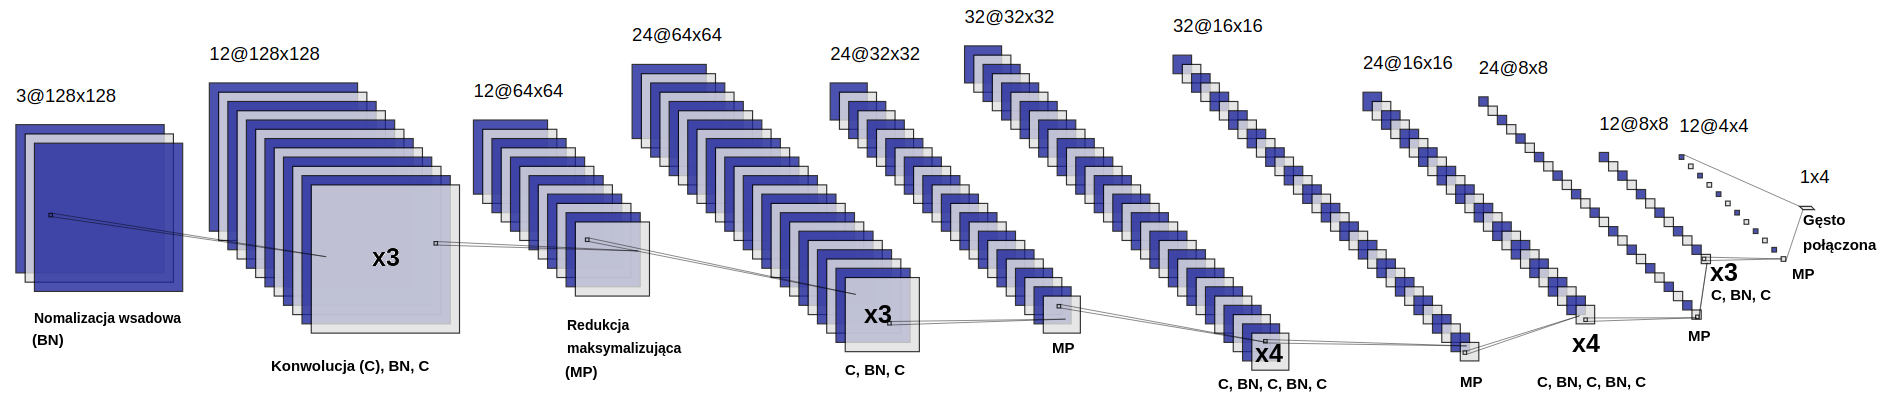
\includegraphics[scale=0.25]{my_model_structure_edited}	
	\caption{Wizualizacja struktury zaproponowanej sieci.}
	\label{fig:ann_visualisation}
\end{figure}

Wyniki skuteczności klasyfikacji architektury z Rys. \ref{fig:ann_visualisation} są niższe niż sieci uprzednio przetrenowanej z powodu znacznie mniejszej sumarycznej liczby danych przepływających przez sieć w trakcie uczenia. Jednak fakt, że ponad połowa próbek została poprawnie zaklasyfikowana (\ref{tab:VGG_1_acc}) oraz nie ma klasy, która byłaby gorzej rozpoznawana niż inne (\ref{tab:VGG_1_params_val}) oznacza, że przy odpowiedniej edycji obecnego modelu można uzyskać wyższe wyniki.

%VGG_1:
 \begin{table}[h!]
\centering
\caption[Short Heading]{Skuteczność modelu VGG16.}
\label{tab:VGG_1_acc}
\begin{tabular}{|c|c|c|c|}
\hline
\textbf{typ zbioru}           & \textbf{treningowy} & \textbf{walidacyjny} & \textbf{testowy} \\ \hline
\textbf{skuteczność {[}\%{]}} & 99                  & 64                   & 53               \\ \hline
\end{tabular}
\end{table}

\begin{table}[h!]
\centering
\caption[Short Heading]{Parametry mierzące jakość klasyfikacji na zbiorze testowym.}
\label{tab:VGG_1_params_val}
\begin{tabular}{|c|c|c|c|c|}
\hline
\textbf{Parametr}                               & \textbf{Precyzja} & \textbf{Czułość} & \textbf{Miara F1} & \textbf{Ilość próbek} \\ \hline
\textbf{klasa eozynofil (E)} & 0.26   & 0.29   & 0.27 & 623  \\ \hline
\textbf{klasa limfocyt (L)} & 0.24  & 0.23 & 0.23  & 620  \\ \hline
\textbf{klasa monocyt (M)} & 0.25   & 0.21    & 0.23  & 620  \\ \hline
\textbf{klasa neutrofil (N)} & 0.26   & 0.28    & 0.27  & 624  \\ \hline
\end{tabular}
\end{table}

Warstwy w architekturze z rozdziału \ref{sec:section_kaggle_1} nie były połączone typowo sekwencyjnie. W co drugiej warstwie konwolucyjnej stosowano rozdzielenie sieci na dwie podsieci o takiej samej liczbie filtrów, ale różnej wielkości jądra, a wyjścia z tych warstw konkatenowano i wsadzano na kolejną warstwę konwolucyjną. Fragment struktury tej sieci obrazuje Rys. \ref{wez_zrob_rysunek_bo_nie_wiem_czy_ktos_sie_domysli_o_co_ci_chodzi}. 


%\begin{figure}[h]
	%\centering
	%\centering
		%\includegraphics[scale=0.25]{wez_zrob_rysunek_bo_nie_wiem_czy_ktos_sie_domysli_o_co_ci_chodzi}	
	%\caption{Wizualizacja struktury sieci z rozdziału \ref{sec:section_kaggle_1}.}	\label{fig:wez_zrob_rysunek_bo_nie_wiem_czy_ktos_sie_domysli_o_co_ci_chodzi}
%s\end{figure}

%ResNet_1
Archiekturą, która także stosuje niesekwencyjne połączenie warstw jest ResNet. OPISAĆ HISTORIĘ ITP. Wejścia są połączone w niej z ze skonktenowanym wjściami warstwy bezpośrednio poprzedzającej oraz warstwy położonej dwa poziomy wcześniej. WRZUCIĆ OBRAZEK ŻEBY BYŁO WIDAĆ O CO CHODZI. Do modelu z Rys. \ref{fig:ann_visualisation} dołączono tego typu połączenia. Wyniki na zbiorze testowym znacząco się poprawiły (\ref{tab:ResNet_1_acc}, \ref{tab:ResNet_1_params_val}).

 \begin{table}[h!]
\centering
\caption[Short Heading]{Skuteczność modelu z cechami ResNet.}
\label{tab:ResNet_1_acc}
\begin{tabular}{|c|c|c|c|}
\hline
\textbf{typ zbioru}           & \textbf{treningowy} & \textbf{walidacyjny} & \textbf{testowy} \\ \hline
\textbf{skuteczność {[}\%{]}} & 99                  & 99                   & 86               \\ \hline
\end{tabular}
\end{table}

\begin{table}[h!]
\centering
\caption[Short Heading]{Parametry mierzące jakość klasyfikacji na zbiorze testowym.}
\label{tab:ResNet_1_params_val}
\begin{tabular}{|c|c|c|c|c|}
\hline
\textbf{Parametr}                               & \textbf{Precyzja} & \textbf{Czułość} & \textbf{Miara F1} & \textbf{Ilość próbek} \\ \hline
\textbf{klasa eozynofil (E)} & 0.23   & 0.22   & 0.23 & 623  \\ \hline
\textbf{klasa limfocyt (L)} & 0.22  & 0.22 & 0.22  & 620  \\ \hline
\textbf{klasa monocyt (M)} & 0.24   & 0.18    & 0.21  & 620  \\ \hline
\textbf{klasa neutrofil (N)} & 0.24   & 0.31    & 0.27  & 624  \\ \hline
\end{tabular}
\end{table}

}
\section{Dobór parametrów}
\label{dobor_parametrow}

\subsection{Ograniczenie przeuczenia modelu}
CNN są sieciami posiadającymi poza warstwami konwolucyjnymi i redukcyjnymi warstwy w pełni połączone (ang. \textit{fully-connected network}). Charakteryzują się one tym, że każdy neuron posiada połączenie z dowolnym innym neuronem w poprzedniej warstwie. To sprawia, że są podatne na zjawisko nadmiernego dopasowania. 
%teraz sposoby jak sobie z tym radzić poza augmentation
%coś o regularyzacji: https://towardsdatascience.com/training-deep-neural-networks-9fdb1964b964, dorzuć podobny obrazek do overfittingu żeby było wiadomo co to
%oraz o bach normalisation: https://towardsdatascience.com/batch-normalization-in-neural-networks-1ac91516821c
